%%%%%%%%%%%%%%%%%%%%%%%%%%%%%%%%%%%%%%%%%
% Design based on a template by Roberto and following the format of
% the xmipp tutorials. In turn, they seem to be based on a template
% from http://www.latextemplates.com
%%%%%%%%%%%%%%%%%%%%%%%%%%%%%%%%%%%%%%%%%

%----------------------------------------------------------------------------------------
%	PACKAGES AND OTHER DOCUMENT CONFIGURATIONS
%----------------------------------------------------------------------------------------

\documentclass[12pt]{article} % Default font size is 12pt, it can be changed here
\usepackage[english]{babel}
\usepackage[utf8]{inputenc}
\usepackage{listings} % To include source code
\usepackage{caption}
\usepackage{geometry} % Required to change the page size to A4
%\geometry{a4paper} % Set the page size to be A4 as opposed to the default US Letter
\usepackage{framed}
\usepackage{url}
\usepackage{graphicx} % Required for including pictures
\usepackage{natbib}
\usepackage{float} % Allows putting an [H] in \begin{figure} to specify the exact location of the figure
\usepackage{hyperref}
\usepackage{menukeys}
\usepackage{array}
\usepackage{fancyhdr}
\usepackage{marvosym}%smileys\Smiley{} \Frowny{}
\usepackage{etoolbox}
\usepackage{listings}
\usepackage{makecell}
\usepackage{marginnote}
\usepackage{soul}
\usepackage[toc,page]{appendix}
\sethlcolor{yellow}

%\renewcommand{\hl}[1]{#1}
%pdflatex -jobname=students '\def\student{}\input{main}'
%pdflatex -jobname=teachers '\def\teachers{}\input{main}'
%  \ifdef{\teachers}
%  {Content for teachers}
%  {Content for students}
\newcommand{\ttt}[1]{\texttt{#1}}
\newcommand{\iii}[1]{\textit{#1}}
\newcommand{\ra}{$\rightarrow$}
\pagestyle{fancy}
\fancyhf{}
\fancyhead[RO]{{Model Building}}
\fancyhead[LO]{Scipion}
%\fancyhead[RO]{{\leftmark}}
\fancyfoot[RO]{\thepage}

\linespread{1.2} % Line spacing

%\setlength\parindent{0pt} % Uncomment to remove all indentation from paragraphs

\newcommand{\scipion}{\textsc{Scipion} }
\newenvironment{command}{\tt\begin{quote}}{\end{quote}}
\newcommand{\comm}[1]{\texttt{#1}}

\newcommand{\imgfig}[3]{\begin{figure}[H]\centering \
\includegraphics[scale=#2]{images/#1} \caption{#3} \end{figure}}

\newcommand{\proto}[1]{\textit{\textbf{#1}}}
\newcommand{\popt}[1]{\textit{#1}}
\newcommand{\pval}[1]{\texttt{#1}}

\newcommand\tstrut{\rule{0pt}{2.4ex}}
\newcommand\bstrut{\rule[-1.0ex]{0pt}{0pt}}

\def \humanAdenoMap {7034}%5172

\begin{document}

%----------------------------------------------------------------------------------------
%	TITLE PAGE
%----------------------------------------------------------------------------------------

\begin{titlepage}

% New command for horizontal lines. Change thickness here.
\newcommand{\HRule}{\rule{\linewidth}{0.5mm}}

\center % Center everything on the page


\includegraphics{images/scipion_logo.png}

{\large Scipion Tutorial Series}\\[1.0cm]

\textsc{\LARGE National Center for Biotechnology}\\[0.5cm]
\textsc{\Large Biocomputing Unit}\\[0.15cm]

\HRule\\[0.4cm]
{ \huge \bfseries Model Building Basic}\\ % Title of your document
\HRule \\[0.5cm]
%{\large \today}\\[3cm] % Date, change the \today to a set date if you want to be precise
\begin{center}
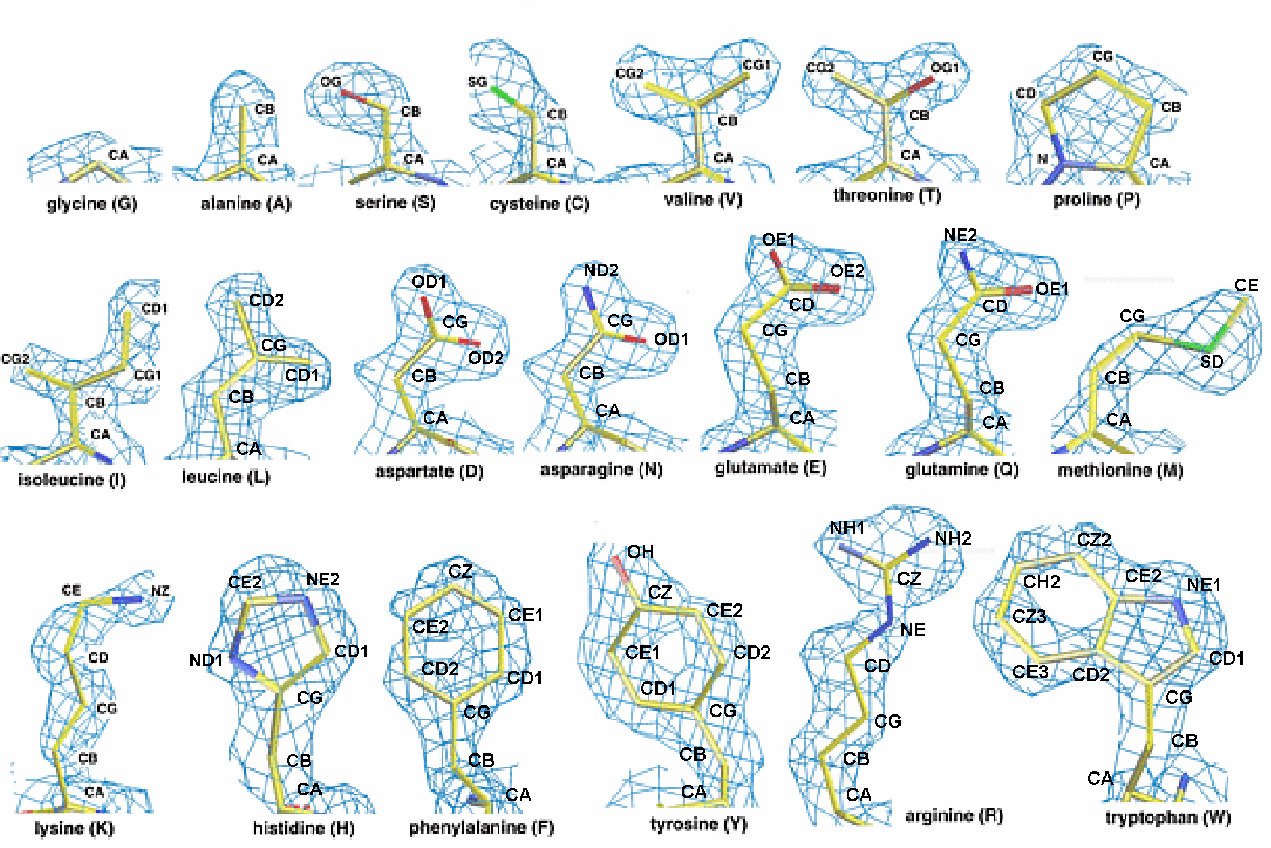
\includegraphics[width=0.70\textwidth]{{images/aadensity}.png}\\
Density for amino acid side chains from an experimental electron density map at 1.5 \AA~resolution (http://people.mbi.ucla.edu/sawaya/m230d/Modelbuilding/modelbuilding.html)\end{center}

%\vfill % Fill the rest of the page with whitespace
%\begin{minipage}{0.4\textwidth}
\begin{flushright}
 \large
%\emph{Author:}\\
  \textsc{Roberto Marabini} % Your name
\end{flushright}
%\end{minipage}

\end{titlepage}


%----------------------------------------------------------------------------------------
%	OBJETIVOS
%----------------------------------------------------------------------------------------


\subsection*{Intended audience}
The recent rapid development of single-particle electron cryo-microscopy (cryo-EM) now allows structures to be solved by this method at resolutions close to 3\AA.  This tutorial provides an introduction to model building for cryo-RM data. %tomography in  electron microscopy with special emphasis in basic image processing. The tutorial requires matlab but does not assume any programing skills. 


\subsection*{We'd like to hear from you}

We have tested and verified the different steps described in this demo
to the best of our knowledge, but since our programs are in continuous
development you may find inaccuracies and errors in this text. Please
let us know about any errors, as well as your suggestions for
future editions, by writing to
\href{mailto:scipion@cnb.csic.es}{scipion@cnb.csic.es}.


\subsection*{Requirements}

This tutorial requires, in addition to $Scipion$,  the \textit{CCP4 suite} including $refmac$ and $coot$ as well as $USCF Chimera$. Basic knowledge of USCF Chimera and $Scipion$ is assumed. Warning: all versions of $refmac$ are not suitable for EM data.

\newpage


%----------------------------------------------------------------------------------------
%	TABLE OF CONTENTS
%----------------------------------------------------------------------------------------

\tableofcontents % Include a table of contents

\newpage % Begins on a new page instead of on the same page as the table of contents


\section{Introduction}

\begin{itemize}
 \item comment on resolution
 \item show full workflow and comment on sub-workflow to b covered
 \item describe model building
\end{itemize}

\section{Particular problem to be solved}
Describe the data and workflow to be used in this tutorial 

 \begin{figure}[H]
 \centering
 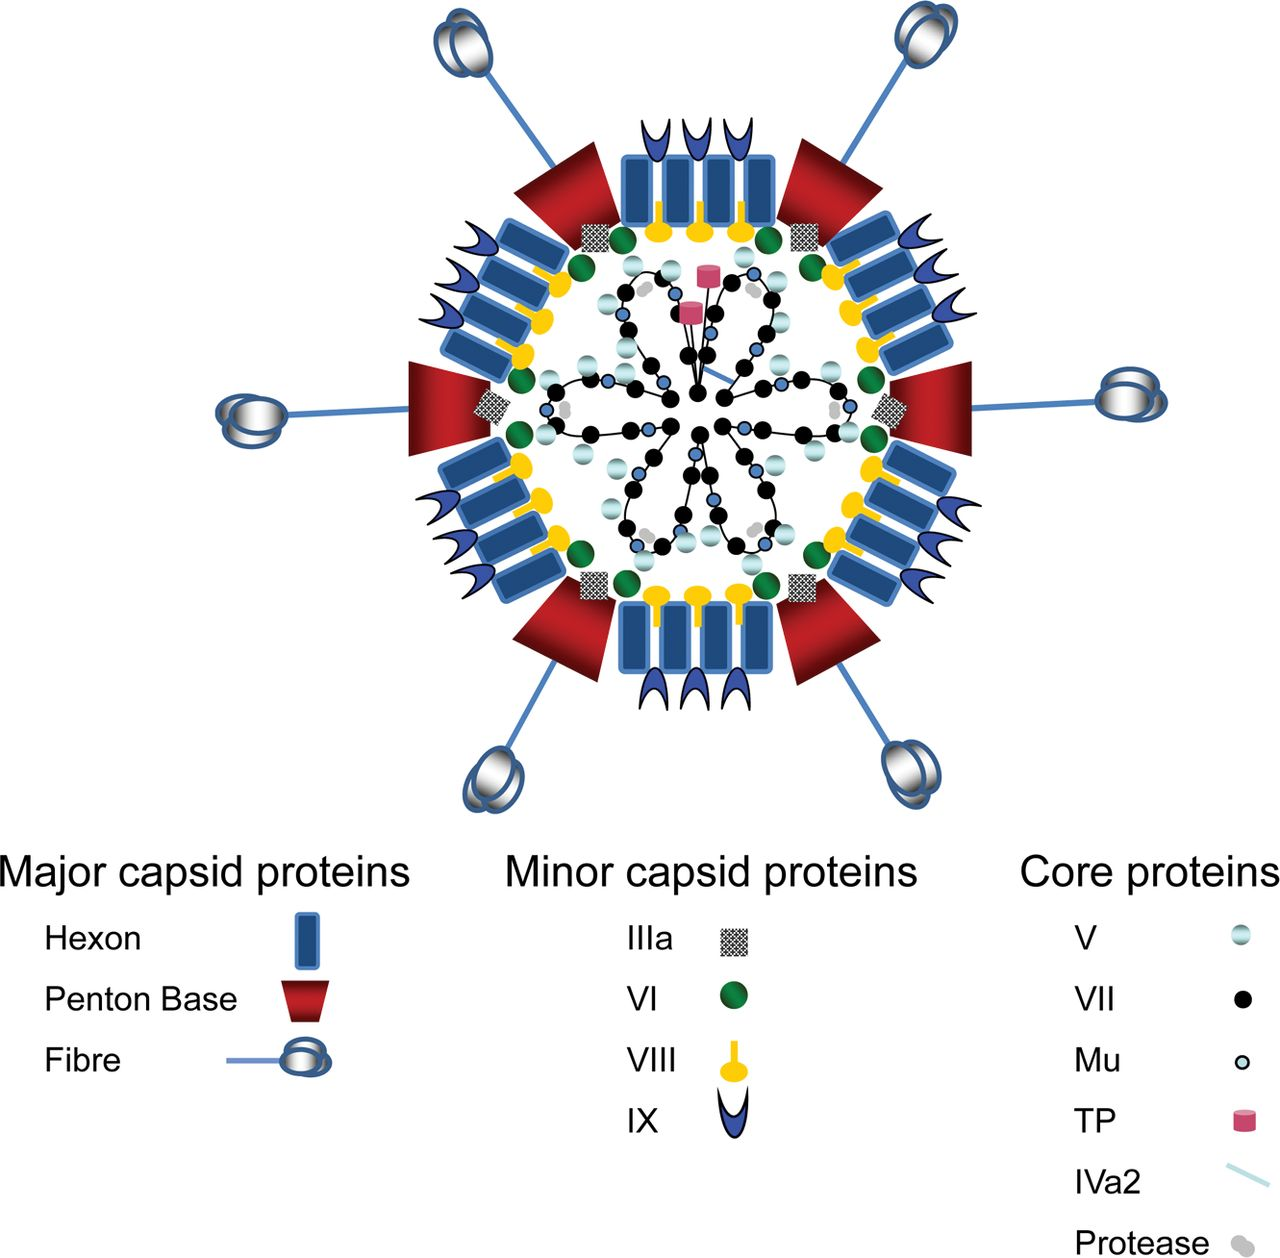
\includegraphics[width=0.7\textwidth]
 {{Images/adeno_scheme}.png}
 \caption{Image example}
 \label{fig:adeno_scheme}
 \end{figure} 
kk
\begin{appendices}
\section{Some Appendix}
\marginnote{swissmodel}[1cm]
When predicting by homology a structure is constructed by aligning a target protein sequence with known template structures. The protein sequence can be obtained from many sources, for example NCBI or UniProt. The quality of a structure depends upon the similarity between the target sequence and the database sharing highest similarity is aligned. 

Esto es otro parrafo
\end{appendices}

\end{document}
